%==================== chapter2_3.tex ====================

\clearpage
\thispagestyle{plain}

\begingroup
\fontsize{16pt}{19.2pt}\selectfont
\justifying
\XeTeXlinebreakskip=0pt plus 1pt minus 0.5pt
\setlength{\parindent}{1.5cm}
\setlength{\parskip}{0pt}

% ---------- การออกแบบเว็บไซต์ที่รองรับการใช้งานบนทุกขนาดของหน้าจอ ----------
\section*{การออกแบบเว็บไซต์ที่รองรับการใช้งานบนทุกขนาดของหน้าจอ (Responsive web design)}
\addcontentsline{toc}{section}{การออกแบบเว็บไซต์ที่รองรับการใช้งานบนทุกขนาดของหน้าจอ (Responsive web design)}

\indent \cite{kinsta2024responsive} การออกแบบเว็บให้รองรับอุปกรณ์หลายชนิด (มือ ถือ แท็บเล็ต เดสก์ท็อป) ด้วยที่อยู่เว็บ
และโค้ดชุดเดียวโดยเลย์เอาต์ปรับตัวตามขนาดหน้าจออัตโนมัติช่วยคงประสบการณ์ใช้งานที่สม่ำเสมอ

\begin{figure}[h]
	\centering
	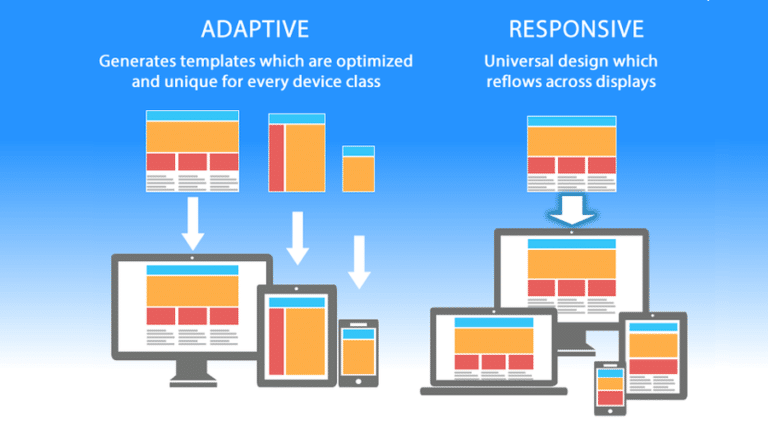
\includegraphics[width=0.8\linewidth]{responsive-adaptive-design-768x425}
	\caption{ภาพตัวอย่าง Responsive web design}
\end{figure}


% ---------- การออกแบบเว็บไซต์ที่รองรับการใช้งานบนทุกขนาดของหน้าจอ ----------

\section*{วงจรการพัฒนาซอฟต์แวร์}
\addcontentsline{toc}{section}{วงจรการพัฒนาซอฟต์แวร์}

\indent วงจรการพัฒนาซอฟต์แวร์ (Software Development Life Cycle: SDLC) มักแบ่งเป็น 6
ขั้นตอน ดังนี้

\begin{enumerate}
	\item \textbf{การวางแผน (Planning)} กำหนดเวลา ขอบเขต ทรัพยากร ผู้มีส่วนเกี่ยวข้อง และความเสี่ยง
	\item \textbf{เก็บรวบรวมและวิเคราะห์ความต้องการ (Requirements)} รวบรวมและทบทวนความต้องการของผู้ใช้/ระบบ
	\item \textbf{ออกแบบซอฟต์แวร์ (Design)} สถาปัตยกรรม ฐานข้อมูล UI/UX ความปลอดภัย เครือข่าย ฯลฯ
	\item \textbf{พัฒนา (Development)} พัฒนาแต่ละฟีเจอร์และรวมเป็นระบบตามดีไซน์
	\item \textbf{ทดสอบ (Testing)} สร้าง Test case ตรวจสอบตาม Requirement และใช้ Automated test ตามความเหมาะสม
	\item \textbf{บำรุงรักษา (Operations \& Maintenance)} เผยแพร่ แก้ไขบั๊ก เพิ่มฟีเจอร์และปรับปรุง คุณภาพอย่างต่อเนื่อง
\end{enumerate}